\section{Introduction}

% A few sentences placing the work in high-level context. Limit it to a few paragraphs at most; your report is on reproducing a piece of work, you don’t have to motivate that work.
This paper presents an attempt to reproduce Diffusion-LM, a language model developed by researchers in the Stanford NLP group. The model is based on continuous diffusions and is capable of solving finer grain control tasks than is possible with current autoregressive language models. This is an important problem because non-autoregressive models have the potential to significantly improve the performance of natural language processing tasks.

The authors of the original paper demonstrate the capabilities of Diffusion-LM through experiments on two datasets: E2E, a dataset consisting of restaurant reviews, and ROCStory, a corpus of short five sentence stories covering a wide range of contexts. These experiments show that Diffusion-LM is able to outperform existing methods on a range of natural language processing tasks.

In this reproduction of the authors' work, I retrained Diffusion-LM from end to end on the E2E dataset and was able to substantiate some of the claims made in the original paper. Despite attempting to do so, I was unable to completely implement the model from scratch in a separate codebase.

\section{Scope of reproducibility}
\label{sec:claims}

The central claim of the paper is that a language model trained via a continuous diffusion process learns hierarchical representations, and that constraints can be placed in this latent space that allow for richer controls than those from autoregressive language models which can only condition text on the left context.

In this paper I attempted to reproduce Diffusion-LM using the model code and without. Using the model code, I planned to investigate the effectiveness of the model in the following fine-grained control tasks:

\begin{itemize}
\item \textbf{Semantic Content}: Given a field and value, generate a sentence that covers the field and value, and report the success rate by exact match of the value.
\item \textbf{Parts-of-speech}: Given a sequence of parts-of-speech tags, generate a sequence of words whose POS tags match the target. Success is measured via word-level exact match.
\item \textbf{Syntax Tree}: Given a target syntactic parse tree, generate text whose syntactic parse matches the given parse. Success is evaluated using F1 scores.
\item \textbf{Syntax Spans}: Given a target pair of span and syntactic category, generate text whose parse tree over the span matches the target syntactic category. Success is measured by the fraction of spans that match exactly.
\item \textbf{Length}: Given a target length, generate a sequence with a length within ±2 of the target.
\item \textbf{Infilling}: Given left and right contexts, generate a sentence that logically connects the two. Both automatic and human evaluation is used for evaluation.
\end{itemize}

\section{Methodology}

% Explain your approach - did you use the author's code, or did you aim to re-implement the approach from the description in the paper? Summarize the resources (code, documentation, GPUs) that you used.

I began by attempting to write my own implementation of the paper, which was challenging due to the scale of the project and time constraints. However, by carefully reading their source code I was able to uncover some details of the authors' implementation that were not mentioned in the paper. My incomplete implementation is included in the github repository to document what I learned along with a working fork of the authors' source code.

Using their source code, I was able to train Diffusion-LM on the E2E dataset. I attempted to train the same model on the ROCStory dataset as well but this model took too long to train and I was unable to fit it within the time constraints for the project.

In my experiments, I found that training Diffusion-LM on the E2E dataset for 200,000 steps took 10 hours on a single NVidia A100 GPU. Training the classifier on the other hand took less time and was feasible on a single consumer GPU. To train the classifier I used a single NVidia RTX 2080 Ti GPU, which took 46 minutes.

\subsection{Model descriptions}

Diffusion-LM is a diffusion model that involves iterative denoising of a Gaussian noise signal. During training, the text is converted into tokens by means of a default BERT tokenizer. These tokens are then embedded into a low-dimensional (e.g. $d=16$ for E2E\cite{novikova2017e2e} and $d=128$ for ROCStories\cite{mostafazadeh2016corpus}) latent space and upsampled by a fully connected network to match a Transformer encoder architecture.

As shown in Figure \ref{fig:graphical-model} from \cite{li2022diffusion}, the token embeddings are iteratively noised according to a schedule parametrized by $q(x_t | x_{t-1}) = \mathcal{N}(x_t; \sqrt{1-\beta_t x_{t-1}}, \beta_t \mathbb{I})$. The $\beta_t$ values are chosen according to a scheduling function such that, after $T=2000$ steps, the resulting embeddings are normally distributed. This forward noise is then reversed by a Transformer model described by the Markov chain: $p_\theta(x_{t-1}|x_t) = \mathcal{N}(x_{t-1}; \mu_\theta(x_t, t), \Sigma_\theta (x_t, t))$.

The noised embeddings are then projected down to $d$ dimensions to match the input embedding size using another fully connected network. This noise removal process is applied to each sample from $x_T$ to $x_0$. A ``rounding step'' $p_\theta (w|x_0)$ is then used to map the resulting embeddings onto the nearest neighboring token using a softmax function.

\begin{figure}[h]
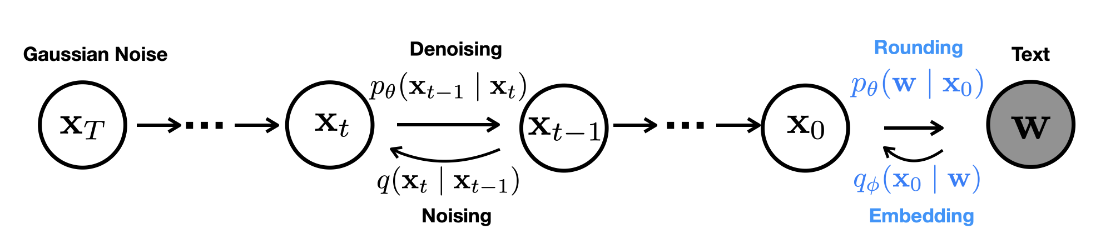
\includegraphics[scale=0.3]{images/diffusion-lm-graphical-model.png}
\centering
\caption{A graphical model representing the forward and reverse diffusion processes. In addition a rounding and embedding mapping is added to shift between continuous latents and the discrete token space.}
\label{fig:graphical-model}
\end{figure}

During training, a clamping trick is employed in which the denoised embeddings are clamped onto the nearest token exactly. This improved the model's stability during training, according to the authors.

The paper considered many different modifications to the diffusion process used during training, exploring hyperparameters such as the latent embedding dimension and different noise schedules. They also employed an analytical simplification of the variational lower bound loss function derived from the widely known image diffusion context.

In the paper, the authors trained two separate diffusion models for the different datasets they considered, and also classifiers for the downstream tasks by running gradient updates on a control objective. In my work, I focused on the E2E model due to time constraints.

Both models were trained end-to-end from scratch using a base bert uncased Transformer\cite{vaswani2017attention} architecture with default parameters. The input and output projection layers employed a single hidden layer of 768 dimensions (matching the embedding dimension of the BERT base model), and a tanh activation function.

\subsubsection{E2E}

For the E2E model, the token embedding dimension was set to 16, and this model was trained for 200,000 steps. When decoding, the authors' subsampled timesteps in order to reduce inference time.

\subsubsection{ROCStories}

For the ROCStories model, the token embedding dimension was 128, and the authors' trained it for 800,000 steps. As a result of these facts, it took much longer to train. The authors' found that subsampling timesteps during inference lead to an unacceptable degradation in the model accuracy.

\subsubsection{Classifier}

Lastly a classifier was trained to run inference on the model over the target tasks. This model takes as input the pre-trained transformer model. In this scenario, the target task is to sample tokens $w$ from a conditional distribution $p(w|c)$ where $c$ is a control variable specific to the task at hand.

We learn this posterior by factorising it into $p(w|c) \propto p_{lm}(w) \cdot p(c|w)$, where $p_{lm}$ is the language model, and $p(c|w)$ is the classifier which we learn from a smaller amount of labelled text data.

\subsection{Datasets}

% For each dataset include
% 1) relevant statistics such as the number of examples and label distributions,
% 2) details of train / dev / test splits,
% 3) an explanation of any preprocessing done, and
% 4) a link to download the data (if available).

The authors trained Diffusion-LM on two datasets, E2E and ROCStories. The E2E dataset consists of 50K restaurant reviews labelled by 8 fields including food type, price and customer rating. The ROCStories dataset consists of 98K five-sentence stories, capturing a rich set of causal and temporal commonsense relations between daily events.

\subsubsection{E2E}

E2E\cite{novikova2017e2e} is a dataset for training end-to-end natural language generation systems in the restaurant domain. It contains 1,026,048 tokens in total with 2,435 unique tokens, an average example length of 20 tokens with the full dataset totalling 12MB. You can download the dataset at \href{https://github.com/tuetschek/e2e-dataset}{https://github.com/tuetschek/e2e-dataset}.

The training set for the E2E dataset contains 42,061 examples, while the validation and test sets contain 4,672 and 4,693 examples respectively. Each example contains a crowdsourced restaurant review paired with a collection of fields and values such as named entities, food type, restaurant type and rating.

\begin{table}
  \centering
  \begin{tabular}{ | m{3cm} | m{7cm}| } 
    \hline
    Name & The Vaults \\ 
    Type & pub \\ 
    Price & more than £ 30 \\
    Customer Rating & 5 out of 5 \\
    Near & Café Adriatic \\
    Text & The Vaults pub near Café Adriatic has a 5 star rating. \\
    \hline
  \end{tabular}
  \caption{Here is one example from the E2E dataset. All values are free text values, but the fields are fixed and not all listed for every example.}
\end{table}

\begin{figure}[h]
  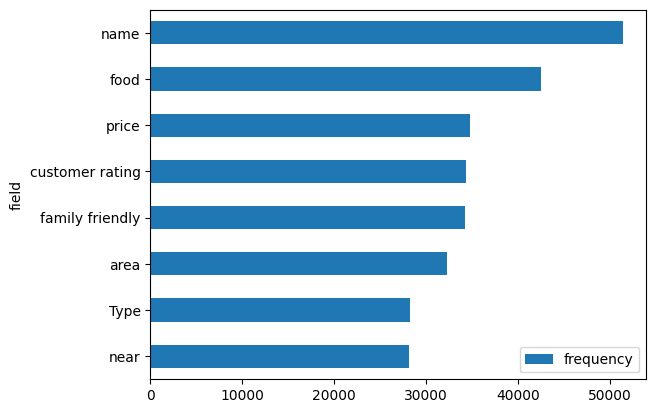
\includegraphics[scale=0.6]{images/e2e-field-frequencies.png}
  \centering
  \caption{In the E2E dataset, the labels occur with the following frequencies}
  \label{fig:e2e-field-frequencies}
\end{figure}

\subsubsection{ROCStories}

The ROCStories\cite{mostafazadeh2016corpus} dataset consists of 98K commonsense five-sentence stories composed by Amazon Mechanical Turk workers. Being the larger dataset at 22.3 MB of text, with the total raw text containing 4,329,367 tokens in total, of which 39,167 are unique. An average example is 44 tokens long. The training set contains 93,161 examples while the validation set contains 5,000 examples.

Because of its size and since it is not restricted to a single domain as E2E is, it is a richer and more complex dataset which makes it more challenging to model. You can download the ROCStories dataset at \href{https://cs.rochester.edu/nlp/rocstories/}{https://cs.rochester.edu/nlp/rocstories/}, and some randomly selected examples are shown in figure \ref{fig:roc-stories-examples}.

\begin{table}
  \centering
  \begin{tabular}{ | m{12cm}| } 
    \hline
    I have a wolf named Kiera, but we nicknamed her Wolfie. She wanted to get up early this morning to go for a walk. She was so excited when she saw a squirrel that she pulled really hard. She almost caught the squirrel, but missed by only a few inches. She was sad when we got home, because she didn't kill the squirrel. \\ \hline
    Katie felt like chicken for lunch. On her lunch break, she left to go to a restaurant. Katie was walking across the lot when a fish hit her on her head. Experts said a sea gull probably dropped the fish while it was flying. Katie thought it was funny until her neck started to hurt. \\ \hline
    I accidentally left the webcam running on my work computer. I discovered it running when I came to work the next morning. I played back the video from the previous evening. On the video I was shocked to find something unusual. It was footage of the cleanup crew eating the apple on my desk! \\
    \hline
  \end{tabular}
  \caption{Here are three randomly selected examples from the ROCStories dataset.}
  \label{fig:roc-stories-examples}
\end{table}

\subsection{Hyperparameters}
% Describe how the hyperparameter values were set. If there was a hyperparameter search done, be sure to include the range of hyperparameters searched over, the method used to search (e.g. manual search, random search, Bayesian optimization, etc.), and the best hyperparameters found. Include the number of total experiments (e.g. hyperparameter trials). You can also include all results from that search (not just the best-found results).

\subsubsection{Diffusion-LM hyperparameters}
Diffusion-LM is a language model that uses a Transformer denoiser with specific hyperparameters, including the number of diffusion steps, the architecture, the embedding dimension, and the noise schedule. In the paper, the authors set the number of diffusion steps to 2000, the architecture to BERT-base, and the sequence length to 64. The embedding dimension was set to 16 for the E2E dataset and 128 for ROCStories. For the noise schedule, they used a sqrt schedule because it was more robust to different model parametrizations and embedding dimensions.

\subsubsection{Training hyperparameters}
To train Diffusion-LM, the authors used the AdamW optimizer with a linearly decaying learning rate initialized at 1e-4, a dropout rate of 0.1, a batch size of 64, and a total number of training iterations of 200,000 for the E2E dataset and 800,000 for the ROCStories dataset.

\subsubsection{Controllable generation hyperparameters}

To control the generation of text with Diffusion-LM, the authors ran gradient updates on the continuous latents of the model. They used the AdaGrad optimizer with a learning rate of 0.0001 and annealed the learning rate at 200,000 steps for the E2E dataset and 400,000 steps for the ROCStories dataset. This allowed them to control the generation of text by updating the latent variables of the model.

\subsection{Experimental setup and code}

% Include a description of how the experiments were set up that's clear enough a reader could replicate the setup.
% Include a description of the specific measure used to evaluate the experiments (e.g. accuracy, precision@K, BLEU score, etc.). 
% Provide a link to your code.

The original authors code was forked at \href{https://github.com/mathematiguy/Diffusion-LM}{https://github.com/mathematiguy/Diffusion-LM} and a Singularity container was built to containerize it fully, including all third party software dependencies. This container is documented in the repository so it can be rebuilt on the users machine, as it is 8 Gigabytes large.

The experiments were separated into training Diffusion-LM separately on the E2E and ROCStories datasets, and then training the classifier for downstream controlled generation tasks.

Instructions are provided so that the reader can build the container locally and then run the experiments on a single node. However in practice we did extra work to deploy the model onto a compute cluster where it can be trained in distributed mode, and these scripts are also provided in case the reader may find them useful.

\subsection{Computational requirements}
% Include a description of the hardware used, such as the GPU or CPU the experiments were run on. 
% For each model, include a measure of the average runtime (e.g. average time to predict labels for a given validation set with a particular batch size).
% For each experiment, include the total computational requirements (e.g. the total GPU hours spent).
% (Note: you'll likely have to record this as you run your experiments, so it's better to think about it ahead of time). Generally, consider the perspective of a reader who wants to use the approach described in the paper --- list what they would find useful.

\subsubsection{Hardware}

While the original paper states that it was possible to train the model on E2E in under 5 hours on  However, we were able to train the model on the E2E dataset successfully, but we found number of hours required for training on our A100 was closer to 10 hours.

\subsubsection{Experiments}

\begin{itemize}
\item \textbf{E2E}: Training Diffusion-LM on the E2E dataset took 10 hours with a single 80GB NVidia A100 GPU.
\item \textbf{ROCStory}: I was unable to train this model, but I would estimate that it should take about 40 hours with a single 80GB A100 GPU.
\item \textbf{Classifier}: I was able to train a single classifier on a consumer grade NVidia RTX 2080 Ti GPU in 45 minutes.
\end{itemize}

We did reach out to the authors to ask if there were details missing from their recommended hyperparameters which could explain this discrepancy, but have not received a reply at present.

\section{Results}
\label{sec:results}

% Start with a high-level overview of your results. Do your results support the main claims of the original paper? Keep this section as factual and precise as possible, reserve your judgement and discussion points for the next "Discussion" section.

With the time and resources I had available I was unable to replicate the results in the paper. Implementing the model from scratch proved to be challenging, due to the level of complexity of the engineering involved and also since the methods for diffusion modelling are not yet well documented across the industry, resulting in a lot of gaps that required some wide reading in order to understand the model as a whole.

Still I was able to get the model running on different architectures and under different scenarios. However unpacking the results of these model runs and assembling them into a report is not possible in remaining time available.

\subsection{Results reproducing original paper}
% For each experiment, say 1) which claim in Section~\ref{sec:claims} it supports, and 2) if it successfully reproduced the associated experiment in the original paper. 
% For example, an experiment training and evaluating a model on a dataset may support a claim that that model outperforms some baseline.
% Logically group related results into sections. 

I was not able to replicate the paper in full, but I was able to train the E2E Diffusion LM model from end to end using a single A100 GPU. So far the only claim I was able to investigate from the original paper was the claim that the model should take 5 hours to train, which I found to be closer to ten hours.


%% \subsubsection{Result 1}

%% \subsubsection{Result 2}

\subsection{Results beyond original paper}

My original interest in this paper came from the possibility that diffusion language models could have applications for learning from noisy text. While I did not have time to do this, I would have been interested in training Diffusion-LM on the noisy output of another model, for example with scanned historical documents.

After conducting this investigation, I was impressed to learn that the model was trained end to end on a relatively small dataset. This is promising for low resource languages, but at the same time noisy text sources have the capacity to be far larger than the training data used for this model. Therefore it may be necessary to simplify the model further so as to speed up the training time on large datasets.
 
%% \subsubsection{Additional Result 1}
%% \subsubsection{Additional Result 2}

\section{Discussion}

Since I was not able to assemble sufficient experimental results, I cannot say whether my work supports or contradicts those made in the paper. My approach proved flawed given my limited time and resources, as I spent too long trying to implement the paper from scratch and this hindered my ability to assemble final results in time.

In spite of this flawed approach, I did learn a lot by studying the paper in detail and this gave me an opportunity to investigate concepts like variational autoencoders, reconstruction loss, propagating gradients through stochastic processes and the reparametrization trick. I hope to be able to use these properly in my work in the future.

I am also satisfied that the codebase I produced may have value to future researchers (or more likely myself) who may seek to reproduce this work. I have collected and packaged the code faithfully into a project that can be deployed locally or on a cluster.

\subsection{What was easy}
% Give your judgement of what was easy to reproduce. Perhaps the author's code is clearly written and easy to run, so it was easy to verify the majority of original claims. Or, the explanation in the paper was really easy to follow and put into code. 

% Be careful not to give sweeping generalizations. Something that is easy for you might be difficult to others. Put what was easy in context and explain why it was easy (e.g. code had extensive API documentation and a lot of examples that matched experiments in papers).

The authors code was easy to run, but also drew heavily from other work on diffusion models from other contexts, such as images. Their code also included the infrastructure necessary to run the model in distributed mode without much modification. The model is also set up to provide logs to weights and biases, so the user can observe the training progress and also GPU utilisation.

The paper also contained a lot of useful detail, and I found the code to be consistent with their stated claims for the model design. The authors also provided the commands necessary to rerun their experiments using their codebase. They were also responsive on their github issues, where I was able to find some useful discussion from people also attempting to adapt the model for their own domains.

\subsection{What was difficult}

% List part of the reproduction study that took more time than you anticipated or you felt were difficult.

% Be careful to put your discussion in context. For example, don't say "the maths was difficult to follow", say "the math requires advanced knowledge of calculus to follow". 

Since the code was written for research, it included many extra details for exploring a wide range of hyperparameters and other small optimization tweaks. Because of this, I attempted to implement the model myself with the idea that a streamlined implementation could be much simpler and have educational value for myself and others.

While the original paper was helpful, I experienced difficulties both when running the authors' code and when attempting to implement the model as described in the paper on my own.

\subsubsection{Original implementation}

Unfortunately, I found that there were many additional details to the model beyond those described in the paper. A significant portion of the code was adapted from other diffusion models that were previously written for controlled image generation.

For example, the paper does not explicitly describe the projection layers used to keep the embedding dimension small, which is necessary for diffusion models to work well. Instead, I had to get these details, and many other small details, from the authors' code. Additionally, the sequential order for the tokens as well as the current diffusion time step were passed to the BERT model using positional embeddings that were added to the input, a step which was not considered worth mentioning in the original paper since it is standard for Transformer models.

However, the primary obstacle to my attempt to follow the original paper's methodology was the implementation details for the diffusion process and the loss function, which used the reparametrization trick to avoid calculating gradients through the stochastic process. The authors borrowed code from another project to implement their diffusion process, but the code was deeply integrated into their implementation, making it difficult to understand exactly how certain things were being computed.

In the end, while I was able to define a forward pass for my version of Diffusion-LM, I was not able to run the backward step due to challenges with the reparametrization trick and the loss function, which required some advanced probability theory to understand.

\subsubsection{Re-running the authors code}

The authors' code ran as described in the readme once I had installed the required dependencies. After I got the original code to run successfully, I attempted to run the model in distributed mode to save time. However, running the model in distributed mode was not documented, so I spent some time searching through the code to figure out how it had been implemented.

Once I had trained the E2E model, I also trained the controlled generation model as well. However, this section of the code required a number of dependencies that were not documented in the repository.

As I mentioned earlier, I found that the E2E model training took twice as long as expected on the same hardware. Getting the models running involved running them many times under different conditions, so this did consume a lot of my time and effort during the attempted reproduction of this work.

\subsection{Communication with original authors}
% Document the extent of (or lack of) communication with the original authors. To make sure the reproducibility report is a fair assessment of the original research we recommend getting in touch with the original authors. You can ask authors specific questions, or if you don't have any questions you can send them the full report to get their feedback before it gets published.

Although I was not able to contact the authors directly, I did watch their 2022 presentation on the paper at NeurIPS. I also found the discussion in their github repository to be lively, as it appears there are many others interested in replicating this work. They responded to many queries there, and reading it helped solve some of my issues.
